\chapter{Recherche}
\label{ch:Recherche}
In diesem Kapitel geht es um mehrere selbstdurchgeführte Befragungen zur Berechtigungsstruktur und der jährlichen Rezertifizierung.
Die jährliche Rezertifizierung ist die Überprüfung, ob die Mitarbeiter ihre Berechtigungen benötigen oder nicht.
Diese wird von den Teamleitern und Führungskräften durch geführt, welche die Berechtigungstruktur nutzen, um dies zu tun.
Dafür wurden drei verschiedene Gruppen befragt.
Die Ergebnisse sind die Grundlage für die Notwendigkeit eines sicheren und übersichlichen Struktur sowie die Festellung der Hauptprobleme der bestehenden Struktur.

\section{Vorgehensweise}
\label{sec:Vorgehensweise}
Für die Befragung wurde erstmal analysiert welche Stakeholder es gibt.
Bei der Analyse wurden die folgenden drei Stakeholder festgestellt:

\begin{itemize}
	\item \ac{FuT}
	\item IT-Systemspezialist
	\item Mitarbeiter
\end{itemize}
Die \ac{FuT} entsprechen den Stakeholdern, die die Berechtigungsstruktur für die jährliche Rezertifizierung nutzen.
Diese haben für eine hohe Priorität, da diese die Berechtigungsstruktur direkt verwenden und für die Sicherheit der Struktur gewähren.
\newline
Die IT-Systemspezialisten sind die Stakeholder, die an der Berechtigungsstruktur gearbeitet haben.
Ebenso wie die Teamleiter und Führungskräfte haben die IT-Systemspezialisten auch eine hohe Priorität, weil diese die Struktur warten und verändern.
\newline
Die Mitarbeiter umfassen das restlichen Arbeitspersonal.
Im Gegensatz zu den anderen beiden Stakeholder haben die Mitarbeiter eine geringe Priorität, da diese weder die Struktur nutzen noch einen anderen Kontakt haben.
\newline
\newline
Nachdem diese drei Stakeholder festgestellt worden sind, wurde spezifisch für diese drei Fragenkataloge entwickelt.
Dabei ist das Ziel festzustellen, welche die größten Probleme aus der Sicht der Teamleiter und Führungskräfte sowie IT-Systemspezialisten gibt.
Die Mitarbeiter wurden befragt, wie viele Berechtigungen diese verfügen, die sie eigentlich nicht mehr brauchen.
Die große Herausforderung besteht dabei, die richtigen Fragen für die Fragenkataloge zu entwerfen.
Die Institution \ac{PRC} hat festgestellt, dass bei geschlossenen Fragen die befragt zu einem großen Teil (über 90\%) eine der vorgeschlagenen Antwortet gewählt haben. \cite{Survey}
Dies stellt ein Problem dar.
Wenn die Fragen zu geschlossen sind, dann kann es dazu führen, dass die befragten nicht die Probleme angeben, die sie sehen.
Auf der anderen Seite sind zu offene Fragen auch eine Herausforderung, da es schwierig wird die verschiedenen Antworten zu quantifizieren und auswerten zu können.
Ebenso ist die Wortwahl ein entscheidener Faktor.
In einer Studie von \ac{PRC} in 2003 wurden die Personen befragt, ob diese für oder den Krieg in Iraq sind, um Saddam Hussein's herrschaft zu beenden.
68\% haben ja gesagt und 25\% für nein.
Darauf wurde die Frage geändert zu, ob diese für oder den Krieg in Iraq sind, um Saddam Hussein's herrschaft zu beenden, selbst wenn es tausende Verluste gibt.
Mit dieser Änderung haben nur noch 43\% dafür gestimmt und 48\% dagegen. \cite{Survey}
\newline
Dies ist relevant, da zum Beispiel bei der Befragung der Mitarbeiter bei einer falschen Formulierung den Gedanken bekommen könnten, dass diese mit der Beantwortung der Frage ihr in Ordnung geben, dass ich ihnen die genannten Berechtigungen entfernen.
Dies kann zu fehlerhaften Ergebnissen führen.
Deshalb müssen die Fragen gut überlegt sein.
\newline
\newline
Für die \ac{FuT} wurden die folgenden Fragen überlegt: 
\begin{itemize}
	\item Wie handhabbar ist für Sie der aktuelle Prozess für die jährliche Rezertifizierung der Vorgangsberechtigung Ihrer Mitarbeiter?
	\item Was finden Sie im aktuellen Rezertifizierungsprozess gut?
	\item Was finden Sie im aktuellen Rezertifizierungsprozess schlecht?
	\item Was würden Sie gerne am aktuellen Rezertifizierungsprozess ändern?
	\item Was halten Sie von der Idee das Profile entweder nur noch (Unter-)Profile oder Profile ausschliesslich Berechtigungen beinhalten?
	\item Soll es eine einheitliche Strukturierung für die Berechtigungsstruktur innheralb der Bereiche geben?
	\item Haben Sie weitere Anmerkungen?
\end{itemize}
Die Fragen wurden größtenteils offen Formuliert, um am besten die Probleme am bestehenden System zu finden.
Dabei umfassen die ersten drei Fragen den Ist-Zustand der Berechtigungstruktur und wie dies die \ac{FuT} finden.
Fragen vier, fünf und sechs wie der Soll-Zustand der Berechtigungstruktur werden soll.
Dabei wurden auch konkrete Vorschläge in den Fragen unterbreitet, um einen erst Eindruck von den \ac{FuT} zu erhalten.
Zum Schluss gab es noch die offene Frage, ob es weitere Anmerkungen gibt, um eventuelle Antworten und Anmerkung zu erhalten, die durch die vorherigen Fragen nicht abgedeckt wurden.
\newline
\newline
Für die IT-Systemspezialisten wurden die folgenden Fragen überlegt: 
\begin{itemize}
	\item Welche Erfahrung haben Sie mit der Berechtigungsstruktur gehabt?
	\item Auf welche Probleme sind Sie im Zusammenhang mit der Berechtigungsstruktur gestoßen?
	\item Gibt es Sachen, die man bei der Berechtigungsstruktur beachten muss?
	\item Haben Sie Vorschläge wie man die Berechtigungsstruktur besser gestalten könnte?
	\item Haben Sie weitere Anmerkungen?
\end{itemize}
Die erste Frage soll dazu Anregen sich über das Thema Gedanken zu bilden, damit die folgenden Fragen einfacher zu beantworten sind.
Dabei soll die zweite Frage klarstellen welche Herausforderungen die befragte Person mit der Struktur hatte.
Dies ermöglicht es dann präventiv gegen diese Vorzugehen und dies direkt mit in die neuen Konzepte zu integrieren.
Bei der dritten Frage sollen mögliche ausnahme Fälle genannt werden, die bei einem Konzept mit berücksichtigt werden müssten.
Anschließend wird gefragt, ob die Person eventuel sich selber Gedanken gemacht hat, welche Möglichkeiten es gibt, um die aktuelle Struktur zu verbessern.
Zum Abschluss wird wieder gefragt, ob es weitere Anmerkung gibt, um falls es solche gibt aber nicht von den vorherigen Fragen abgedeckt wurde.
\newline
\newline
Die Mitarbeiter haben die Frage bekommen:
\newline
\newline
\textit{Wie viele Vorgangsberechtigungen in der Produktion Sie im Hoblink haben, die Sie nicht mehr nutzen?}
\newline
\newline
Bei dieser Frage ware es wichtig diese so zu formulieren, dass die befragte Person nicht den Eindruck bekommt, dass ich ihr die Berechtigungen wegnehmen möchte.
Dies würde ansonsten zu fehlerhaften Ergebnissen führen.
Die Befragung der Mitarbeiter dient dazu, um die Problematik der nicht optimalen Berechtigungsstruktur darzustellen und auch um feste Zahlen zu haben.
\newline
\newline
Dabei wurden die \ac{FuT} in der Informatikabteilung befragt, da diese am ehesten Kontakt mit der Berechtigungstruktur haben.
Andere \ac{FuT} außerhalb der Informatik wurden nicht befragt, weil die Wahrscheinlichkeit zu gering ist zum zeitlichen Aufwand.
Bei den IT-Systemspezialisten wurden alle Personen befragt, die mir bekannt waren.
Von den Mitarbeitern wurden zufällig von jedem Team von jeder Abteilung einer befragt.
Dies soll dazu dienen, dass man das Ergebnis skalieren kann.
\newpage
\section{Auswertung}
\label{sec:Auswertung}

Die folgenden Graphiken zeigen die Antworten der jeweiligen Befragungen.

\begin{figure}[h!]
 \centering
 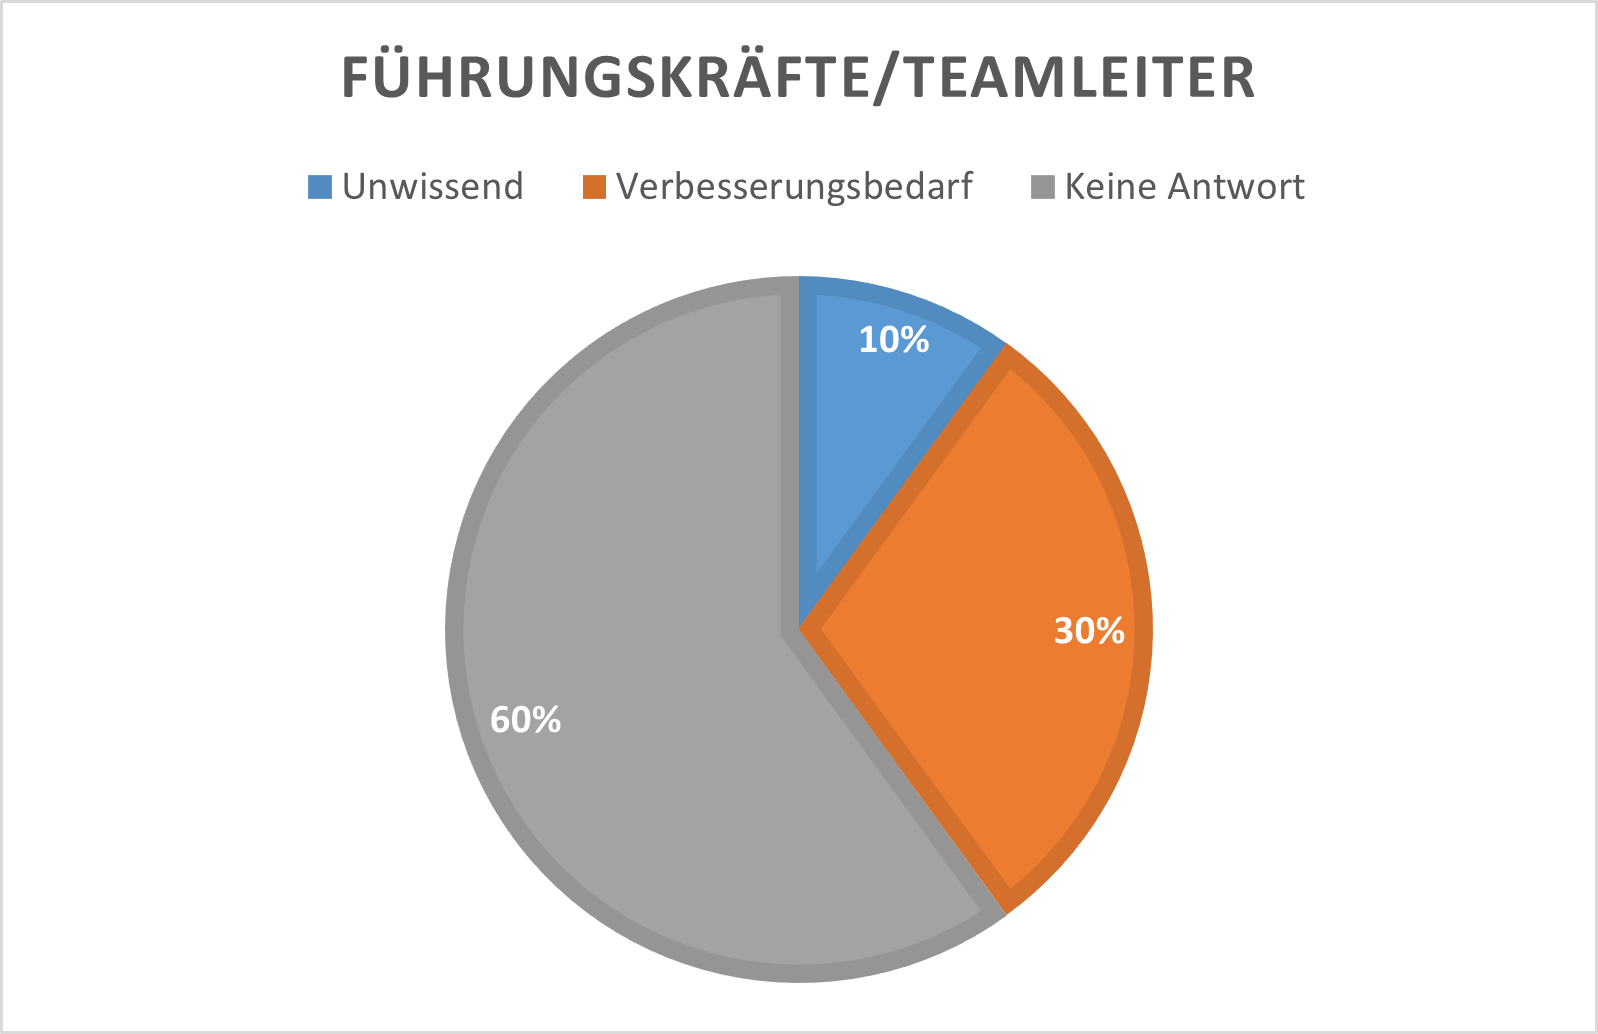
\includegraphics[width=1\textwidth]{gfx/Picture/FuT.PNG}
 \caption{Auswertung der Ergebnisse von den \ac{FuT}}
 \label{fig:Fut}
\end{figure}
\begin{figure}[h!]
 \centering
 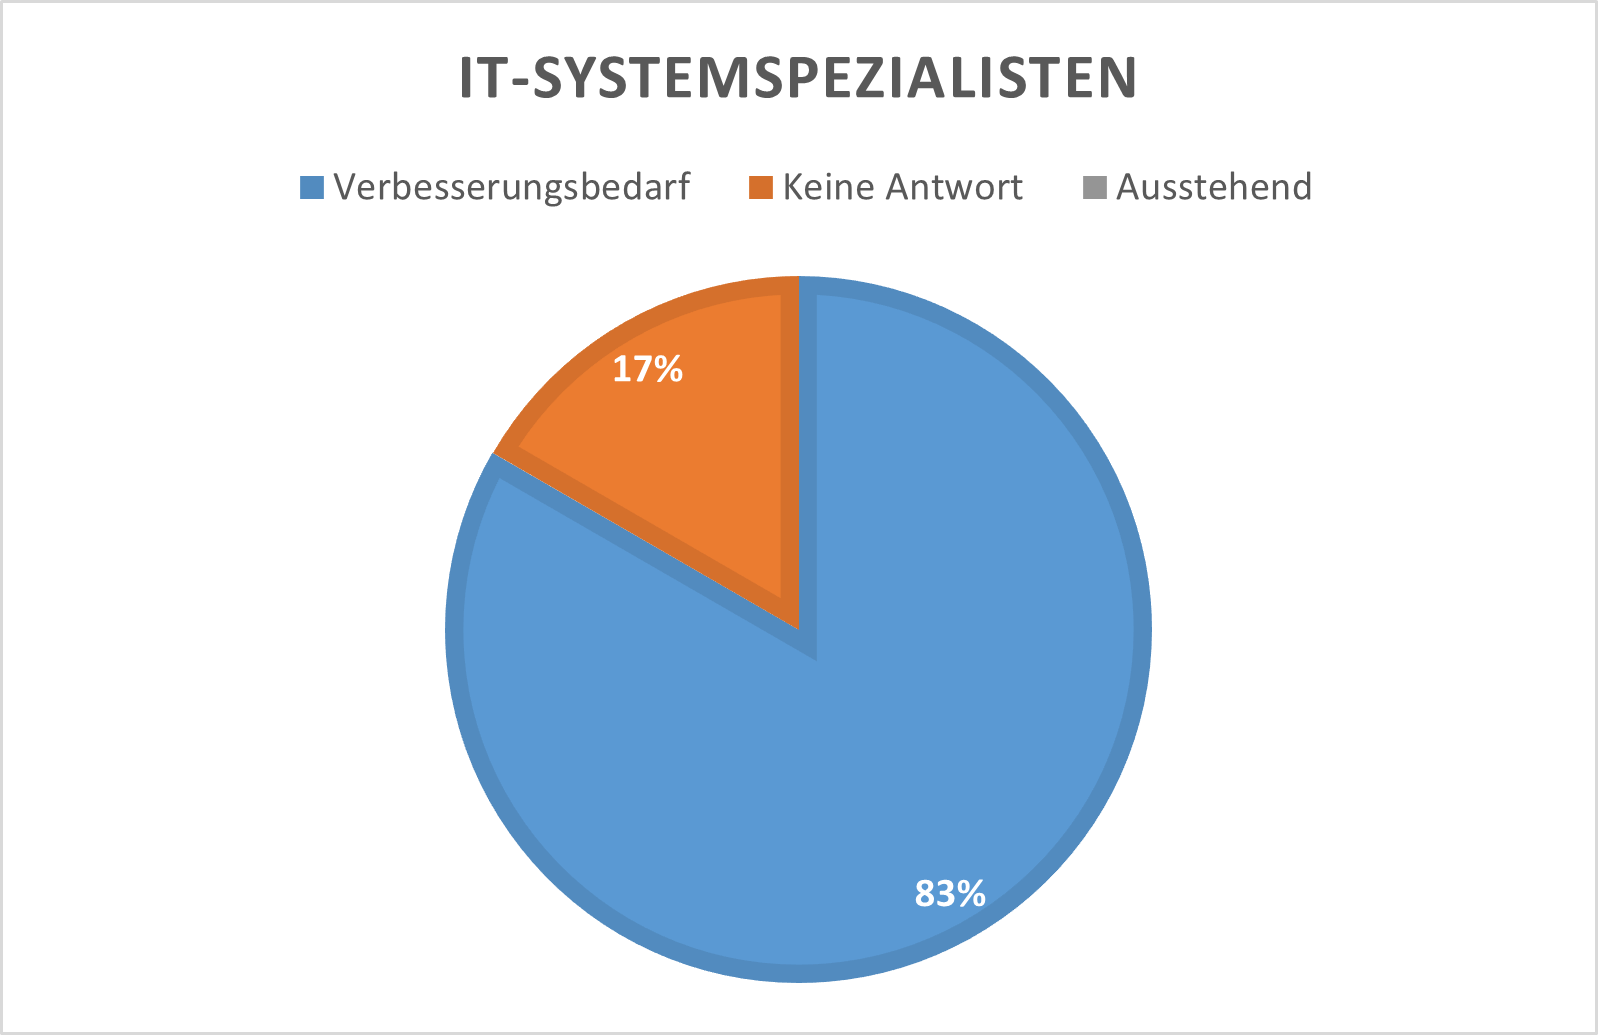
\includegraphics[width=1\textwidth]{gfx/Picture/IT.PNG}
 \caption{Auswertung der Ergebnisse von den IT-Systemspezialisten}
 \label{fig:IT}
\end{figure}
\begin{figure}[h!]
 \centering
 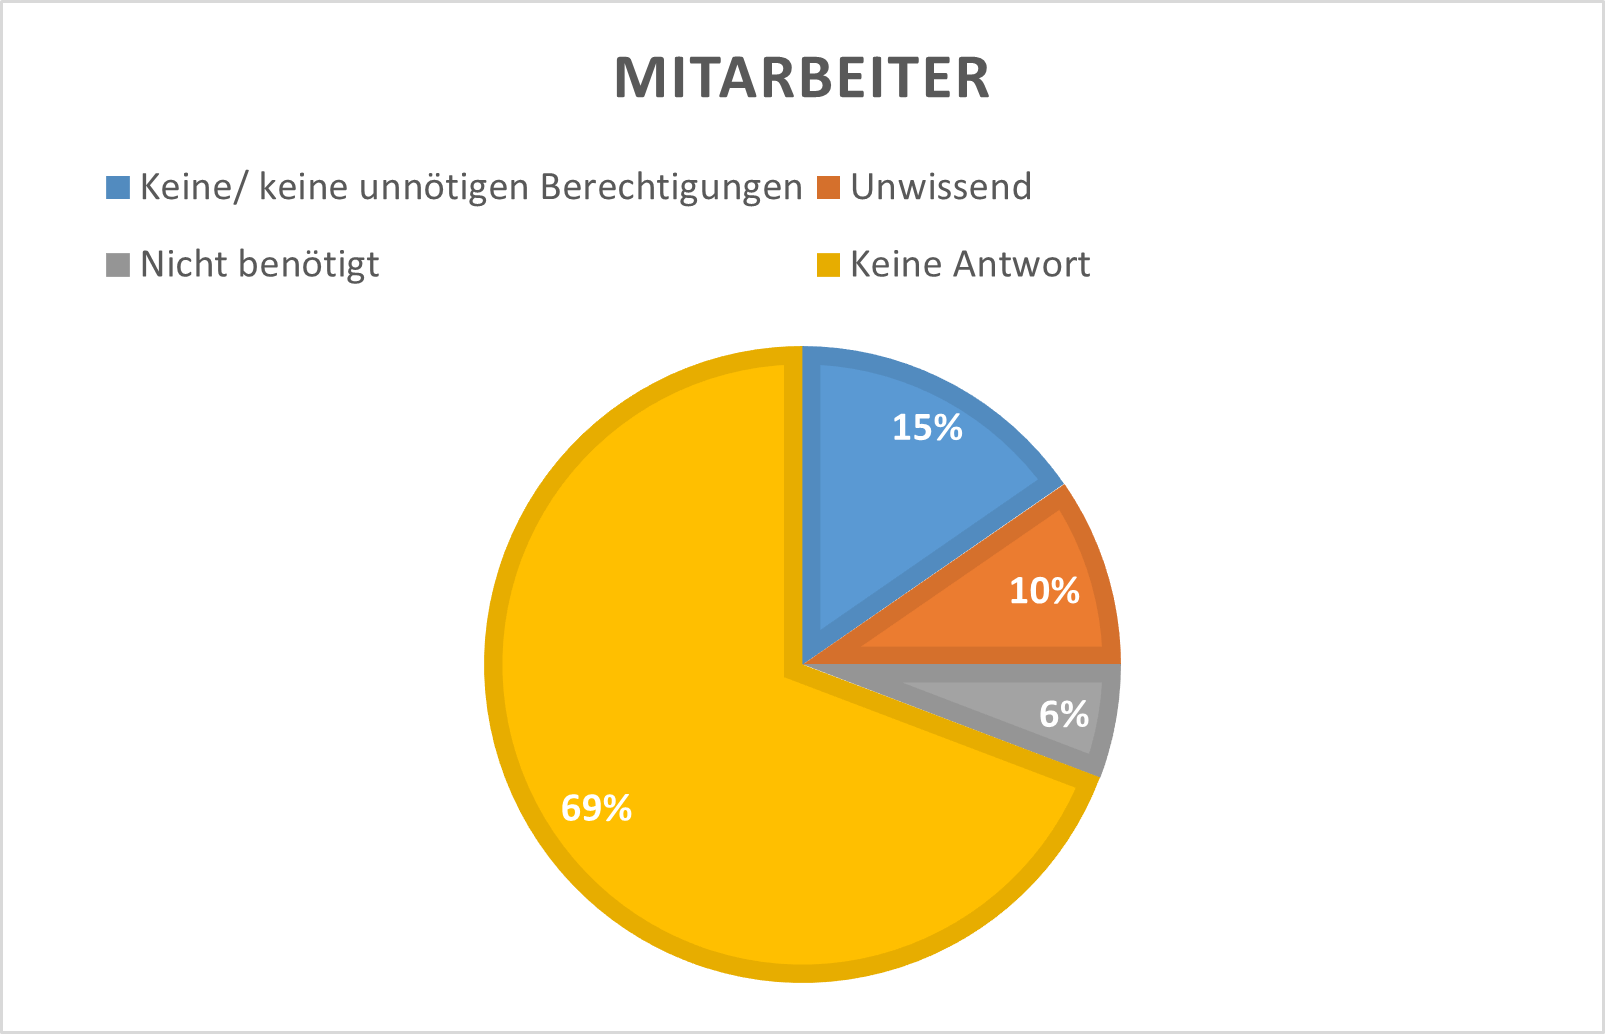
\includegraphics[width=1\textwidth]{gfx/Picture/Mitarbeiter.PNG}
 \caption{Auswertung der Ergebnisse von den Mitarbeitern}
 \label{fig:Mit}
\end{figure}
\newpage
Von den zehn befragten Teamleitern (Graphik \ref{fig:Fut}) haben vier davon an der Umfrage teilgenommen.
Von diesen vier haben drei angegeben, dass sie mit der aktuellen Struktur und Vorgehen umgehen können, es aber Verbesserungsbedarf besteht.
Dabei haben sie folgende Vorschläge gemacht:

\begin{itemize}
	\item Veraltete Vorgänge entfernen
	\item Helvetia Leben braucht keine HV/HI Mandaten
	\item Nur Änderung zum Vorjahr vergleichen
	\item Überprüfung von Sachgebieten anstelle von Profilen/Vorgängen
\end{itemize}

Der erste Punkt wird aktuell sukzessive umgesetzt, ist jedoch nicht einfach und dauert lange.
Die Helvetia Versicherung ist aufgrund von gesetzlichen Regelungen in die Helvetia Leben und Helvetia Komposit aufgeteilt.
Dabei umfasst Helvetia Leben alle Versicherungen für die Person.
Dazu verfügt die Helvetia über drei Mandaten (HV, HI und HL).
Der HV Mandat wird für den Zugriff von deutschen Daten verwendet.
HI im Gegensatz ist der Mandat für internationale Informationen.
Helvetia Leben hat explizit den HL Mandaten.
Deswegen wurde vorgeschlagen, dass die Helvetia Leben Mitarbeiter nicht die anderen beiden benötigen.
Jedoch ist dies nicht umsetztbar, da es Fälle gibt bei denen diese auf die anderen Daten zugreifen müssen.
Zum Beispiel wenn ein Vermittler nach Daten fragt, die nur über den HV Mandaten verfügbar sind, muss der Mitarbeiter in der Lage sein, diese zu zugreifen.
\newline
Der Vorschlag, dass man nur Änderung zum Vorjahr vergleicht würde den Aufwand massiv reduzieren, würde aber nicht mehr den Sinn der jährlichen Rezertifizierung erfüllen.
Das Problem dabei besteht, dass ein Mitarbeiter nach mehreren Jahren eine Berechtigungen nicht mehr benötigt.
Wenn man dann nur den Vergleich zum Vorjahr betrachtet, würde diesem nie die Berechtigungen entzogen werden.
\newline
Die Überprüfung mittels Sachgebiete anstelle von Profilen/Vorgängen findet aktuell schon statt, da der Aufwand bei der Überprüfung der indivduellen Profilen/Vorgängen zu groß wäre.
Zudem bestände dann auch die große Wahrscheinlichkeit, dass versehentlich gewisse Profile/Vorgänge übersehen werden, welche eigentlich entfernt werden müssten.
\newline
\newline
Von den IT-Systemspezialisten haben sechs von sieben an der Befragung (\ref{fig:IT}) teilgenommen.
Im Interview mit den Befragten Personen haben diese verschiedene Anmerkung zum bestehenden System gegeben:

\begin{itemize}
	\item Chaotisch hiercheraufbau
	\item Intransparent
	\item Schreckliches durcheinander
\end{itemize}

Wie man an den Bemerkung erkennen kann, sehen die IT-Systemspezialisten das größte Problem bei der Hierarchie und dem Aufbau der Struktur.
Dabei haben sie verschiedene Vorschläge gemacht wie man die Struktur aus ihrer Sicht verbessern kann.

\begin{itemize}
	\item Transparenter gestalten
	\item Baumstruktur "`verdammen"'
	\item Profile in Profile abschaffen
	\item Eindeutige Struktur
	\item Konventionen
\end{itemize}
Auch wurde angesprochen, ob man das bestehende System nicht in RACF auslagern könnte.
Dabei wurde erwähnt, dass man sich darüber schonmal gedanken gemacht hat.
Dies wird weiter im Kapitel (\ref{sec:chapter05:racF}) eingegangen.
Zudem haben sie auch einen eigenen Lösungsidee vorgeschlagen.
Dieser wird in (\ref{sec:chapter04:minimal}) erläutert.
\newline
\newline
Bei der Umfrage (\ref{fig:Mit}) von den Mitarbeitern haben 16 von 52 geantwortet.
Dabei haben sechs Personen angeben, dass diese über gar keine oder keine unnötigen Berechtigungen verfügen.
Fünf haben geschrieben, dass dies nicht sicher sind und andere fünf haben angegeben, dass diese über Berechtigungen verfügen, die sich eigentlich nicht bräuchten.
Nachdem ich die Ergebnisse der Personen ausgewertet habe, habe ich mir von ein paar Personen die Berechtigungen angesehen und habe dies mit ihren Aussagen verglichen.
Dabei habe festgestellt, dass zwei Personen die angegeben haben, dass diese über gar keine Berechtigungen verfügen und den Host nicht verwenden, über Berechtigungen verfügen.
Da diese nicht über diese Berechtigungen wissen, kann angenommen werden, dass diese nicht benötigen, weil ansonsten diese bei der Umfrage gelogen haben.
\newline
\newline
[Eventuell wird hier noch was eingefügt. Werde die Person fragen, damit es wissenschaftlicher ist]
\newline
\newline
Wenn man dies Berücksichtigt ändert sich der Graphen (\ref{fig:Mit}) wie folgt.
\begin{figure}[h!]
 \centering
 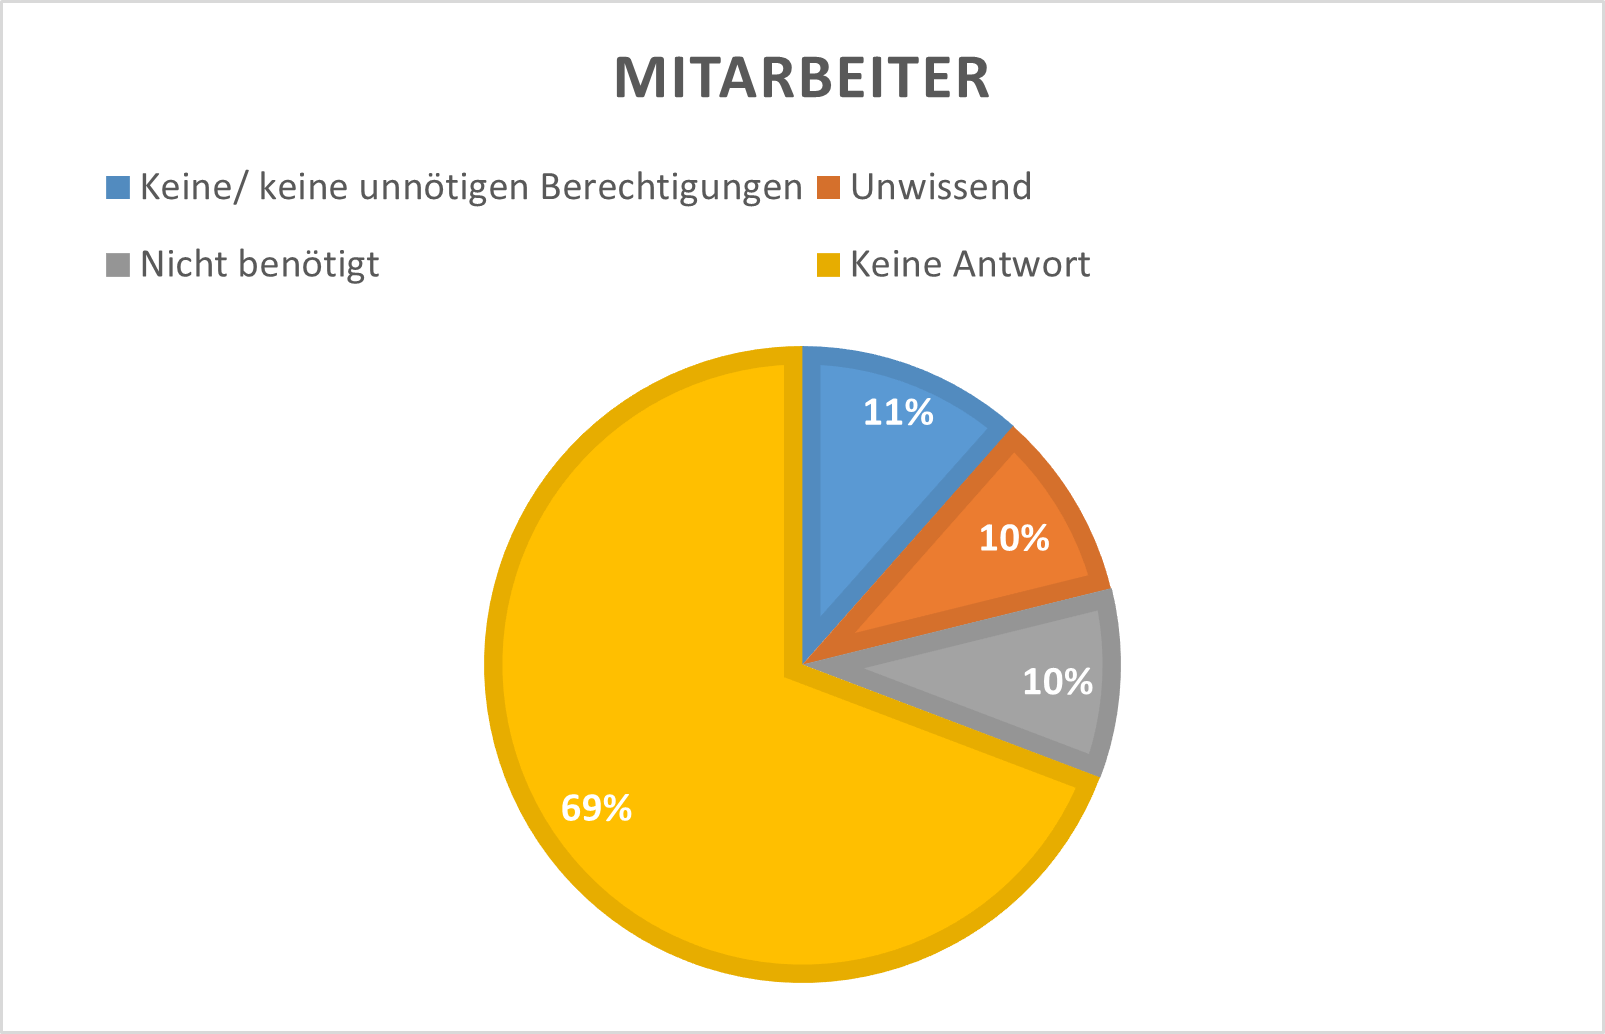
\includegraphics[width=1\textwidth]{gfx/Picture/Mitarbeiter(korregiert).PNG}
 \caption{Auswertung der Ergebnisse von den Mitarbeitern nach der Überprüfung}
 \label{fig:MitPruf}
Wenn man jetzt die Graphik betrachtet kann man erkennen, dass von den Personen die geantwortet haben 33\% zu viele Berechtigungen haben.

\end{figure}
\section{Ergebnis}
\label{sec:Ergebnis}